\section{Micro architecture}

This section details the internal structure and behavior of the module. The design into constituent sub-modules. A detailed block diagram is often effective here.

\subsection{Module hierarchy}
% Present a clear hierarchical breakdown of the design into its constituent sub-modules.

\begin{itemize}[nosep]
    \item \textbf{SPI Slave Interface}: Central controller interfacing with the external SPI Master and internal blocks.
    \item \textbf{Deserializer}: Sub-module for serial-to-parallel conversion of incoming data.
    \item \textbf{Serializer}: Sub-module for parallel-to-serial conversion of outgoing data.
    \item \textbf{CRC Block}: Sub-module for error detection and correction, integrated with both incoming and outgoing data paths.
    \item \textbf{APB Bus Interface}: Connects low-frequency logic to the rest of the system (note: detailed integration with high-frequency components to be covered in a broader system report).
    \item \textbf{Addresser}: Intermediate module responsible for organizing data packets and providing them to the APB Master, including the implementation of address auto-increment.
    \item \textbf{APB Master}: Implements the master side of the APB communication protocol to interact with external APB Slaves. It receives operational information from the Addresser and generates protocol signals to manage read or write transactions with the selected Slave, including the PENABLE signal to enable the access phase.
    \item \textbf{APB Slave}: Represents the slave side of the APB communication protocol interface, which is outside the deliverable scope of the BioQuick module but documented for validation purposes. It interacts with the APB Master via protocol signals for memory access operations.
\end{itemize}

\subsection{Sub-Module Functionality}

This subsection provides detailed descriptions of each submodule, including their inputs, outputs, control signals, and datapath. These details are crucial for design verification and integration, clearly defining interaction points and signal roles.

\subsubsection{SPI Slave Interface}
The SPI Slave Interface handles SPI protocol logic for configuration and transaction timing, forwarding data to Deserializer/CRC for write operations and from Serializer for read operations. It outputs a status signal to indicate ongoing transactions.

\begin{table}[!htb]
    \centering
    \caption{SPI Slave Interface Signals}
    \label{tab:spi-slave-interface-signals}
    \begin{tabular}{|m{.10\columnwidth}|m{.2\columnwidth}|m{.60\columnwidth}|}
        \hline
        \textbf{Signal} & \textbf{Signal} & \multirow{2}{*}{\textbf{Description}} \\
        \textbf{Type} & \textbf{Name} & \\
        \hline
        Input & clk & System clock for low-frequency operations (up to 1 MHz) \\
        Input & sck & SPI clock from external master \\
        Input & ss & Slave select signal from external master \\
        Input & mosi & Master Out Slave In data line for receiving serial data \\
        Input & cpol & Clock polarity configuration (0 = idle low, 1 = idle high) \\
        Input & cpha & Clock phase configuration (0 = sample on leading edge, 1 = trailing edge) \\
        Input & bit\_order & Bit transmission order (0 = MSB first, 1 = LSB first) \\
        Output & miso & Master In Slave Out data line for transmitting serial data \\
        Output & spi\_busy & Status signal indicating ongoing transaction (1 = busy, 0 = idle) \\
        \hline
    \end{tabular}
\end{table}

\textbf{Datapath Description}: Serial data received on MOSI is forwarded to the Deserializer for conversion to parallel format during write operations, while parallel data from the Serializer is transmitted serially on MISO during read operations. The submodule coordinates timing based on SCK and SS signals, adhering to configuration settings (cpol, cpha, bit\_order).

\subsubsection{Deserializer}
The Deserializer processes serial input bit-by-bit into a 16-bit shift register, outputting parallel data to a synchronization register and comparator for further processing, supporting burst handling.

\begin{table}[!htb]
    \centering
    \caption{Deserializer Signals}
    \label{tab:deserializer-signals}
    \begin{tabular}{|m{.10\columnwidth}|m{.2\columnwidth}|m{.60\columnwidth}|}
        \hline
        \textbf{Signal} & \textbf{Signal} & \multirow{2}{*}{\textbf{Description}} \\
        \textbf{Type} & \textbf{Name} & \\
        \hline
        Input & clk & System clock for low-frequency operations \\
        Input & sck & SPI clock for serial data sampling \\
        Input & ss & Slave select signal to control burst handling \\
        Input & i\_mosi & Serial data input from SPI Slave Interface \\
        Input & bit\_order & Bit transmission order (0 = MSB first, 1 = LSB first) \\
        Output & data\_block[15:0] & 16-bit parallel data output to synchronization register and comparator \\
        \hline
    \end{tabular}
\end{table}

\textbf{Datapath Description}: Serial data from mosi\_data is shifted into a 16-bit register bit-by-bit, following the specified bit\_order. Once complete, the full 16-bit data block is output to a synchronization register for further processing or comparison, with burst handling managed via the ss signal.

\subsubsection{Serializer}
The Serializer serializes parallel data into serial output for MISO transmission, supporting burst handling.

\begin{table}[!htb]
    \centering
    \caption{Serializer Signals}
    \label{tab:serializer-signals}
    \begin{tabular}{|m{.10\columnwidth}|m{.2\columnwidth}|m{.60\columnwidth}|}
        \hline
        \textbf{Signal} & \textbf{Signal} & \multirow{2}{*}{\textbf{Description}} \\
        \textbf{Type} & \textbf{Name} & \\
        \hline
        Input & clk & System clock for low-frequency operations \\
        Input & sck & SPI clock for serial data transmission \\
        Input & ss & Slave select signal to control burst handling \\
        Input & parallel\_data[7:0] & 8-bit parallel data input for serialization \\
        Input & crc\_code[7:0] & 8-bit CRC code to append to data \\
        Input & bit\_order & Bit transmission order (0 = MSB first, 1 = LSB first) \\
        Output & o\_miso & Serial data output to SPI Slave Interface for MISO transmission \\
        \hline
    \end{tabular}
\end{table}

\textbf{Datapath Description}: Parallel data and CRC code, signals (parallel\_data[7:0]) and (crc\_code[7:0]), are combined and shifted out bit-by-bit as miso\_data, following the specified bit\_order. The serialization process is timed by SCK, with burst handling managed via the ss signal.

\subsubsection{CRC Block}
The CRC Block generates 8-bit CRC codes using the CRC\&CCITT algorithm from bit-by-bit input, used for validation in write operations and appending in read operations. The decision to use a single CRC block for both functions is detailed in the 'Design Choices and Justifications' subsection (see Section~\ref{sec:design-choices}).

\begin{table}[!htb]
    \centering
    \caption{CRC Block Signals}
    \label{tab:crc-block-signals}
    \begin{tabular}{|m{.10\columnwidth}|m{.2\columnwidth}|m{.60\columnwidth}|}
        \hline
        \textbf{Signal} & \textbf{Signal} & \multirow{2}{*}{\textbf{Description}} \\
        \textbf{Type} & \textbf{Name} & \\
        \hline
        Input & clk & System clock for low-frequency operations \\
        Input & data\_bit & Single bit input for CRC calculation (from MOSI or parallel data) \\
        Input & reset & Reset signal to initialize CRC calculation \\
        Output & crc\_code[7:0] & 8-bit CRC code output for validation or appending \\
        Output & crc\_error & Error signal indicating CRC mismatch during validation (1 = error, 0 = valid) \\
        \hline
    \end{tabular}
\end{table}

\textbf{Datapath Description}: During write operations, incoming data bits (data\_bit) are processed to generate a CRC code (crc\_code[7:0]) for validation against received CRC. During read operations, data bits are used to generate a CRC code to append to outgoing data. A crc\_error signal is asserted if a mismatch is detected during validation.

\subsubsection{Addresser}
The Addresser manages the accumulation and delivery of essential data to the APB Master to facilitate memory access, supporting address auto-increment for sequential operations.

\begin{table}[!htb]
    \centering
    \caption{Addresser Signals}
    \label{tab:addresser-signals}
    \begin{tabular}{|m{.10\columnwidth}|m{.2\columnwidth}|m{.60\columnwidth}|}
        \hline
        \textbf{Signal} & \textbf{Signal} & \multirow{2}{*}{\textbf{Description}} \\
        \textbf{Type} & \textbf{Name} & \\
        \hline
        Input & clk & System clock for high-frequency operations (100 MHz) \\
        Input & i\_ss & Slave select signal to initiate data accumulation \\
        Input & data[15:0] & 16-bit data package input from low-frequency domain \\
        Output & o\_addr[11:0] & 12-bit address output to APB Master for memory access \\
        Output & o\_data[15:0] & 16-bit data output to APB Master for write operations \\
        Output & o\_rw & Operation type (0 = read, 1 = write) to APB Master \\
        Output & Transfer & Control signal to initiate data transfer to APB Master \\
        Output & PSSTRB[1:0] & Strobe signals indicating valid data bytes for APB Master \\
        \hline
    \end{tabular}
\end{table}

\textbf{Datapath Description}: The Addresser receives 16-bit data packages (data[15:0]) and reorganizes them into address (o\_Addr[11:0]) and data (o\_data[15:0]) components for the APB Master. It determines the operation type (o\_rw) and supports auto-increment of addresses for sequential memory operations, using the signals Transfer and PSSTRB[1:0].

\subsubsection{APB Master}
The APB Master implements the master side of the APB communication protocol, coordinating memory access transactions with external APB Slaves. It ensures transaction timing and data integrity as per the protocol specification. The BioQuick module's scope includes the APB Master functionality up to the communication interface.

\begin{table}[!htb]
    \centering
    \caption{APB Master Signals}
    \label{tab:apb-master-signals}
    \begin{tabular}{|m{.10\columnwidth}|m{.2\columnwidth}|m{.60\columnwidth}|}
        \hline
        \textbf{Signal} & \textbf{Signal} & \multirow{2}{*}{\textbf{Description}} \\
        \textbf{Type} & \textbf{Name} & \\
        \hline
        Input & clk & System clock for high-frequency operations (100 MHz) \\
        Input & o\_addr[11:0] & 12-bit address input from Addresser \\
        Input & o\_data[15:0] & 16-bit data input from Addresser for write operations \\
        Input & o\_rw & Operation type input from Addresser (0 = read, 1 = write) \\
        Input & Transfer & Control signal from Addresser to initiate transfer \\
        Input & PSSTRB[1:0] & Strobe signals from Addresser indicating valid data bytes \\
        Input & PREADY & Status input from external APB Slave indicating transaction completion \\
        Input & PSLVERR & Status input from external APB Slave indicating transaction error \\
        Input & PRDATA[15:0] & 16-bit read data input from external APB Slave \\
        Output & PWRITE & Operation type output as per APB protocol (0 = read, 1 = write) \\
        Output & PADDR[11:0] & 12-bit address output as per APB protocol \\
        Output & PWDATA[15:0] & 16-bit write data output as per APB protocol \\
        Output & PENABLE & Control signal as per APB protocol to enable access phase \\
        Output & PSELx & Control signal as per APB protocol to select specific APB Slave \\
        \hline
    \end{tabular}
\end{table}

\textbf{Datapath Description}: The APB Master receives address, data, and operation details from the Addresser, translating them into APB protocol signals (PWRITE, PADDR, PWDATA, PENABLE, PSELx) to communicate with an external APB Slave. It manages transaction timing according to the protocol, awaiting PREADY and PSLVERR responses, and forwards read data (PRDATA) back to the system for further processing.

\subsubsection{APB Slave}
The APB Slave represents the slave side of the APB communication protocol interface. It is documented here for validation purposes, but it is explicitly outside the deliverable scope of the BioQuick module. The module's scope ends at the APB Master's communication interface, which interacts with external APB Slaves via the protocol.

\begin{table}[!htb]
    \centering
    \caption{APB Slave Signals (External Interface for Validation)}
    \label{tab:apb-slave-signals}
    \begin{tabular}{|m{.10\columnwidth}|m{.25\columnwidth}|m{.55\columnwidth}|}
        \hline
        \textbf{Signal} & \textbf{Signal} & \multirow{2}{*}{\textbf{Description}} \\
        \textbf{Type} & \textbf{Name} & \\
        \hline
        Input & PCLK & System clock for high-frequency operations (100 MHz) \\
        Input & PRESETn & Reset signal for initialization (active low) \\
        Input & PADDR[11:0] & 12-bit address input as per APB protocol from APB Master \\
        Input & PWDATA[15:0] & 16-bit write data input as per APB protocol from APB Master \\
        Input & PWRITE & Operation type input as per APB protocol (0 = read, 1 = write) \\
        Input & PENABLE & Control signal as per APB protocol to enable access phase \\
        Input & PSELx & Control signal as per APB protocol to select this slave \\
        Output & PRDATA[15:0] & 16-bit read data output as per APB protocol to APB Master \\
        Output & PREADY & Status signal as per APB protocol indicating transaction completion \\
        Output & PSLVERR & Status signal as per APB protocol indicating transaction error \\
        Output & WRITE\_ENABLE & Control signal for memory write operations (implementation dependent) \\
        \hline
    \end{tabular}
\end{table}

\textbf{Datapath Description}: As an external entity, the APB Slave is expected to receive operation commands from the APB Master via protocol signals (PADDR, PWDATA, PWRITE, PENABLE, PSELx). For write operations, it may use a signal like WRITE\_ENABLE to store data at the specified address. For read operations, it retrieves data from memory and outputs it as PRDATA. Transaction status is communicated back via PREADY and PSLVERR signals as per the APB protocol. Note that the implementation details of the APB Slave are outside the BioQuick module's scope.

\subsection{Data and control flow}

\begin{itemize}[nosep]
    \item \textbf{SPI Receive Flow}: Serial data enters via SPI Slave Interface (MOSI), driven by sck (up to 1 MHz). It is sent to both Deserializer for conversion to parallel format (data\_block[15:0]) and CRC Block for CRC generation (crc\_code[7:0]). The Deserializer outputs to a synchronization register and comparator (with data\_block[15:8] for CRC comparison), and the CRC Block outputs to the comparator. If valid, data transitions to a sync device for high-frequency processing. The received data may follow one of two paths: a write operation or a read operation.
    
    \item \textbf{Write Operation Flow}: Following synchronization of the data in the high-frequency domain, the information block is stored in the Addresser. If the operation type is designated as a write, the information is reorganized to furnish the APB Master with the requisite data for a write operation. Upon receiving two 16-bit blocks, the transfer signal is activated, enabling the APB Master to initiate its data transfer to the APB Slave. The APB Slave receives the address and the data to be written from the APB Master, subsequently returning the PREADY signal to the APB Master upon completion, thereby concluding the write cycle.
    
    \item \textbf{Read Operation Flow}:Following package synchronization, the information block is stored in the Addresser. If the operation type is a read, once the Addresser receives the address and operation details, the transfer signal is initiated, allowing the APB Master to capture the information and issue a read request to the APB Slave. The Slave responds to the Master through the PRdata[15:0] bus with the data from the specified address. The Master then propagates this data to a FIFO Sync module, which transfer it to the low-frequency block. Parallel data (parallel\_data[7:0]) from an async FIFO or other source is sent to the Serializer, while CRC Block generates crc\_code[7:0] from bit-by-bit data. The Serializer converts and transmits combined data via SPI Slave Interface (MISO).
    
    \item \textbf{Control Signals}: SPI Slave Interface manages ss, cpol, cpha, bit\_order, and spi\_busy. Control signals coordinate Deserializer/Serializer data processing and CRC generation/validation, with burst handling based on ss state.
\end{itemize}

\subsection{Diagrams and Waveforms}

Refer to Fig.~\ref{fig:low-freq-flow} for a visual representation of the architecture and interconnections for the low-frequency architecture. Additional diagrams for critical submodules are provided or planned to illustrate detailed interfaces and data flow.

\begin{itemize}[nosep]
    \item \textbf{SPI Slave Interface Diagram}: A detailed diagram focusing on SPI signal interactions is planned to complement the signal table and datapath description.
    % \item \textbf{SPI Slave Interface Diagram}: A detailed diagram focusing on SPI signal interactions is planned as Fig.~\ref{fig:spi-interface-diagram} to complement the signal table and datapath description.
    \item \textbf{Addresser Data Flow Diagram}: Fig.~\ref{fig:AddressFlow} already illustrates the data organization and flow within the Addresser, supporting its detailed signal description.
    \item \textbf{APB Protocol Interaction Diagrams}: Fig.~\ref{fig:APBDiagram} and Fig.~\ref{fig:APBSlaveFlow} illustrate the APB communication protocol signal interactions from the master perspective and the expected external slave responses, respectively. These diagrams focus on protocol flow rather than physical components, with signal tables providing further clarity. Note that the BioQuick module's scope ends at the APB Master interface.
\end{itemize}

% \begin{figure}[!htb]
%     \centering
%     \includegraphics[width=1\linewidth]{figures/spi_interface_diagram.png}
%     \caption{SPI Slave Interface Diagram (Placeholder)}
%     \label{fig:spi-interface-diagram}
% \end{figure}

% TODO: Replace using the draw-io
% State-Transition Diagrams: To define the behavior of finite state machines (FSMs).
% Timing Diagrams or Behavioral Waveforms: To show the sequence and timing of signals at key interfaces.
        
\begin{figure}[!htb]
    \centering
    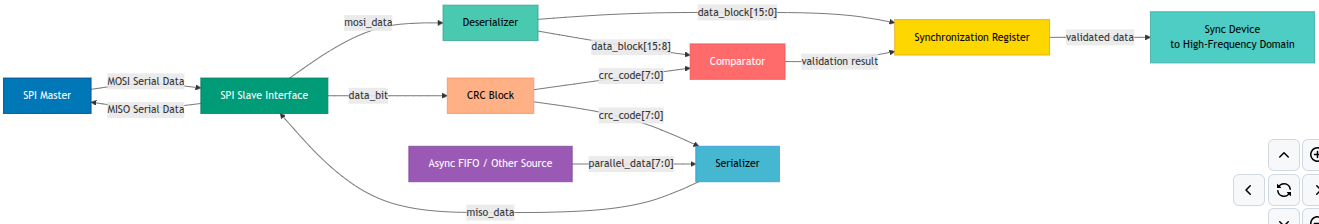
\includegraphics[width=1\linewidth]{figures/lowfreq_flow.png}
    \caption{SPI data flow}
    \label{fig:low-freq-flow}
\end{figure}

The Fig.~\ref{fig:high-freq-flow} illustrates the data flow and communication architecture within a high-frequency system designed for memory access operations. 

\begin{figure}[!htb]
    \centering
    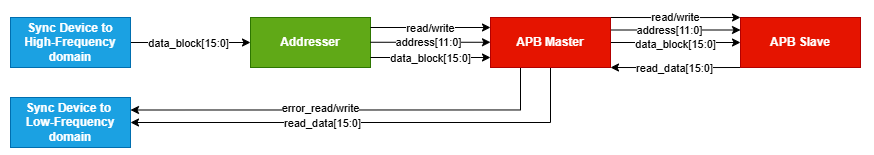
\includegraphics[width=1\linewidth]{figures/highfreq_flow_crop.png}
    \caption{High frequency data flow}
    \label{fig:high-freq-flow}
\end{figure}

The APB Master implements the master side of the AMBA 4 APB protocol, and its protocol signal interactions are illustrated in Fig.~\ref{fig:APBDiagram}.

\begin{figure}[!htb]
    \centering
    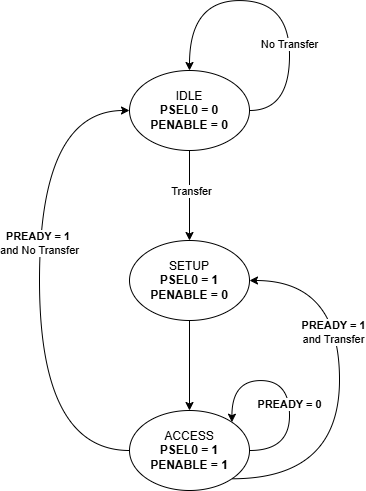
\includegraphics[scale=0.372]{figures/APBdiagramcrop.png}
    \caption{APB Protocol Signal Flow (Master Perspective)}
    \label{fig:APBDiagram}
\end{figure}

To illustrate the expected operational flow of an external APB slave as per the protocol, Fig.~\ref{fig:APBSlaveFlow} presents the behavior for managing memory access transactions. Note that the APB Slave implementation is outside the BioQuick module's deliverable scope.

\begin{figure}[!htb]
    \centering
    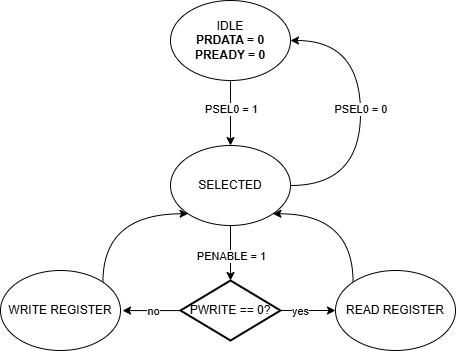
\includegraphics[scale=0.5]{figures/APBslaveFlow.png}
    \caption{APB Protocol Interaction (External Slave Perspective)}
    \label{fig:APBSlaveFlow}
\end{figure}

The Addresser organizes and accumulates data packets, and its data flow is presented in Fig \ref{fig:AddressFlow}.

\begin{figure}[!htb]
    \centering
    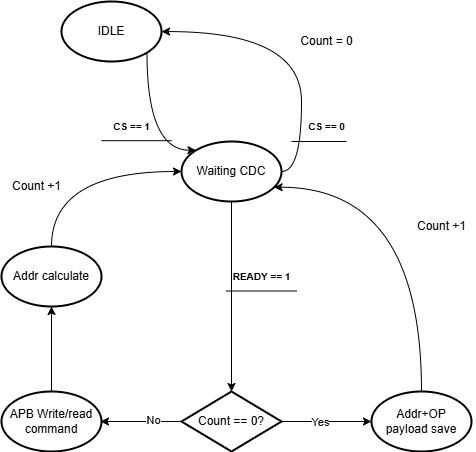
\includegraphics[scale=0.5]{figures/AddressDataFlow.png}
    \caption{Addresser diagram.}
    \label{fig:AddressFlow}
\end{figure}

Additionally, a Finite State Machine (FSM) diagram for control logic is provided in Section \ref{sec:operation}.

\subsection{System-Level Inputs and Outputs}

This subsection provides a holistic view of the BioQuick module's top-level inputs and outputs, detailing how the module interacts with external components.

\begin{table}[!htb]
    \centering
    \caption{BioQuick Module System-Level Signals}
    \label{tab:system-level-signals}
    \begin{tabular}{|m{.10\columnwidth}|m{.2\columnwidth}|m{.60\columnwidth}|}
        \hline
        \textbf{Signal} & \textbf{Signal} & \multirow{2}{*}{\textbf{Description}} \\
        \textbf{Type} & \textbf{Name} & \\
        \hline
        Input & clk & System clock for low-frequency operations (up to 1 MHz) \\
        Input & PCLK & System clock for high-frequency operations (100 MHz) \\
        Input & reset & Reset signal for low-frequency domain initialization \\
        Input & PRESETn & Reset signal for high-frequency domain initialization (active low) \\
        Input & sck & SPI clock from external master for low-frequency communication \\
        Input & ss & Slave select signal from external master to initiate transactions \\
        Input & mosi & Master Out Slave In data line for receiving serial data \\
        Input & cpol & Clock polarity configuration for SPI (0 = idle low, 1 = idle high) \\
        Input & cpha & Clock phase configuration for SPI (0 = sample on leading edge, 1 = trailing edge) \\
        Input & bit\_order & Bit transmission order for SPI (0 = MSB first, 1 = LSB first) \\
        Output & miso & Master In Slave Out data line for transmitting serial data \\
        Output & spi\_busy & Status signal indicating ongoing SPI transaction (1 = busy, 0 = idle) \\
        \hline
    \end{tabular}
\end{table}

\textbf{Interaction Description}: The BioQuick module interfaces with an external SPI Master through signals like sck, ss, mosi, and miso, with configuration options (cpol, cpha, bit\_order) defining communication parameters. Dual clocks (clk for low-frequency, PCLK for high-frequency) and reset signals (reset, PRESETn) manage operations across domains. The spi\_busy output provides feedback on transaction status. Internal synchronization mechanisms handle data transfer between domains, which are detailed in respective submodule descriptions.

\subsection{Design Choices and Justifications}\label{sec:design-choices}

This subsection outlines specific design decisions made during the development of the BioQuick module, distinguishing them from project requirements to provide transparency in the design rationale. These choices are justified based on technical constraints, optimization goals, and compatibility considerations.

\begin{itemize}[nosep]
    \item \textbf{Single CRC Block for Validation and Generation}:
        \begin{itemize}[nosep]
            \item \textbf{Decision}: A single CRC block is utilized for both validation of incoming data during write operations and generation of CRC codes for outgoing data during read operations.
            \item \textbf{Justification}: This design choice optimizes resource usage by reusing the same hardware for both functions, reducing area and power consumption on the chip. It aligns with the project constraint of minimizing complexity in the low-frequency domain while maintaining robust error detection capabilities using the CRC\&CCITT algorithm.
        \end{itemize}
    \item \textbf{4-bit Operation Field Format (1-bit Operation Type Extended by 3 Zeros)}:
        \begin{itemize}[nosep]
            \item \textbf{Decision}: The operation field in the data format is defined as 4 bits, with 1 bit indicating the operation type (0 for read, 1 for write) and the remaining 3 bits set to zero.
            \item \textbf{Justification}: This format ensures compatibility with SPI communication constraints, providing a simple and clear distinction between operation types while reserving space for potential future extensions. It balances the need for a compact data packet with clarity in command interpretation, facilitating efficient parsing by the SPI Slave Interface.
        \end{itemize}
    \item \textbf{16-bit Data Packages with 12-bit Address}:
        \begin{itemize}[nosep]
            \item \textbf{Decision}: Data packages are structured as 16-bit entities, with 12 bits allocated for addressing in memory operations.
            \item \textbf{Justification}: This structure supports a sufficient address space for the targeted memory operations while keeping data transfers aligned with common word sizes in digital systems, optimizing data handling efficiency between low and high-frequency domains.
        \end{itemize}
\end{itemize}

These design choices are distinct from project mandates such as the operational frequency (up to 1 MHz for low-frequency components) and the use of SPI for communication, which are predefined requirements. Cross-references to this subsection are included in relevant parts of the documentation to clarify the basis for specific implementations.

\subsection{Naming Convention Guideline}

To ensure consistency across the documentation, the following naming conventions are applied to signal names:
\begin{itemize}[nosep]
    \item Signal names are in lowercase to maintain readability (e.g., 'mosi', 'sck').
    \item Underscores are used for multi-word names (e.g., 'bit\_order', 'spi\_busy').
    \item Prefixes indicate signal direction where applicable (e.g., 'i\_' for input signals like 'i\_mosi', 'o\_' for output signals like 'o\_miso').
    \item Protocol-specific signals follow standard capitalization (e.g., APB signals adhere to AMBA conventions like 'PADDR', 'PWRITE').
\end{itemize}
This guideline is applied throughout the documentation to enhance clarity and uniformity.

\subsection{Bar Sizing Standard for Diagrams}

To maintain visual consistency in diagrams, bit-width representations follow a uniform standard:
\begin{itemize}[nosep]
    \item 1-bit signals are represented with a thin line or notation (e.g., '1b').
    \item 8-bit signals use a medium-width line or notation (e.g., '8b').
    \item 16-bit and above signals use a thicker line or notation (e.g., '16b').
\end{itemize}
This standard applies to all figures (e.g., Fig.~\ref{fig:low-freq-flow}, Fig.~\ref{fig:high-freq-flow}) to ensure consistent visual representation of data buses and signal widths. Updates to diagrams will align with this standard as needed.

\subsection{Instantiation and integration}

To instantiate these components into a higher-level design, connect the SPI Slave Interface to the external SPI Master pins (MOSI, MISO, SCK, SS) and provide configuration inputs (cpol, cpha, bit\_order), system clocks (clk for low-frequency, PCLK for high-frequency), and reset signals (reset, PRESETn). The output from the synchronization register should connect to a sync device for high-frequency domain interfacing, and the async FIFO or other data source should feed into the Serializer for read operations. Detailed connectivity and clock enables will be specified in the complete system integration documentation.
